\chapter*{Lecture 17}
\begin{recall}{}{}
\begin{itemize}
\item Auxiliary equations
\end{itemize}
\end{recall}




\section*{Auxiliary equation} 

\subsection{Two real, distinct roots: $b^2-4ac>0$}
[last class]
\subsection{Two complex, distinct roots: $b^2-4ac<0$}
In this case, our root equation can be written as :

\begin{equation*}
r=-\frac{b}{2a}\pm \frac{1}{2a}\sqrt{b^2-4ac}=\underbrace{-\frac{b}{2a}}_{\alpha}\pm \underbrace{\frac{1}{2a}\textcolor{red}{\sqrt{4ac-b^2}}}_\beta \underbrace{i}_{\sqrt{-1}}=\alpha\pm\beta i
\end{equation*}

The resulting solutions take the form:
\begin{equation*}
e^{r_1x}=e^{(\alpha+\beta i)x} \qquad e^{r_2x}=e^{(\alpha-\beta i)x}
\end{equation*}

We recall the Euler formula ("the most remarkable formula in mathematics", Feynman)
\begin{equation}
e^{ix}=\cos(x)+i \sin(x)
\end{equation}
Using this formula, we find that our solutions become:
\begin{align*}
e^{(\alpha+\beta i)x}=e^{\alpha x}\left(\cos(\beta x)+i\sin(\beta x)\right)\\
e^{(\alpha-\beta i)x}=e^{\alpha x}\left(\cos(\beta x)-i\sin(\beta x)\right)
\end{align*}
We now add together and divide by 2 these solutions to obtain $y_1$:
\begin{equation*}
y_1=0.5(e^{\alpha x}\left(\cos(\beta x)+i\sin(\beta x)\right)+e^{\alpha x}\left(\cos(\beta x)-i\sin(\beta x)\right))=e^{\alpha x}\cos(\beta x)
\end{equation*}

Subtract together the same two equations and divide by $2i$ these solutions to obtain $y_2$:
\begin{equation*}
y_2=\frac{1}{2i}(e^{\alpha x}\left(\cos(\beta x)+i\sin(\beta x)\right)-e^{\alpha x}\left(\cos(\beta x)-i\sin(\beta x)\right))=e^{\alpha x}\sin(\beta x)
\end{equation*}

Therefore, the general solution takes the form:
\begin{equation}
\boxed{y_{general}=e^{\alpha x}\left(c_1\cos(\beta x)+c_2\sin(\beta x)\right)}
\end{equation}






\begin{center}
\noindent\rule{4cm}{0.4pt}
\end{center}


\begin{exmp}{Auxiliary equation (two imaginary, distinct roots):}\\
Solve:
\begin{equation*}
9y''+6y'+4y=0
\end{equation*}
Solution: \\
We have a constant coefficient homogeneous equation therefore, we can solve with the auxiliary equation:
\begin{equation*}
9r^2+6r+4=0
\end{equation*}
such that:
\begin{equation*}
\alpha = -b/2a=-1/3 \qquad \beta=\frac{1}{2a}\sqrt{4ac-b^2}=\frac{1}{\sqrt{3}}
\end{equation*}

The linearly independent solutions are:
\begin{equation*}
y_1=e^{\alpha x}\cos(\beta x) \qquad y_2=e^{\alpha x}\sin(\beta x)
\end{equation*}
The general solution:

\begin{equation*}
y_{general}=e^{-x/3}\left[c_1 \cos(\frac{x}{\sqrt{3}})+c_2 \sin(\frac{x}{\sqrt{3}})\right]
\end{equation*}
\end{exmp}

\begin{center}
\noindent\rule{4cm}{0.4pt}
\end{center}

%
%\subsection{Two real, but equal roots: $b^2-4ac=0$}
%If  $b^2-4ac=0$, our root equation yields: $r=r_1=r_2=-b/(2a)$ or $2ar+b=0$.
%
%This gives us ONE solution to the ODE of the form:
%\begin{equation*}
%y_1=e^{rx}=e^{-b/(2a) x}
%\end{equation*}
%How can we find the second solution?????
%Answer: using the reduction of order technique.
%\begin{align*}
%y_2&=V(x)y_1=V(x)e^{r x}\\
%y'_2&=V'(x)e^{r x}+rV(x)e^{rx}\\
%y''_2&=V''(x)e^{r x}+r^2V(x)e^{rx}+rV'(x)e^{rx}\\
%\end{align*}
%
%Sub into the general form of the ODE:
%\begin{equation}
%aV''+\underbrace{(2ar+b)}_{=0\text{ by definition}}V'+\underbrace{(ar^2+br+c)}_{\text{auxiliary equation} =0}V=0
%\end{equation}
%So we obtain:
%\begin{equation*}
%V''=0 \qquad V=Ax+B
%\end{equation*}
%Therefore, our second solution takes the form (we can drop the constants!):
%\begin{equation*}
%y_2=V y_1=x e^{rx}=xy_1
%\end{equation*}
%
%We can obtain the general form of the solution as:
%\begin{equation}
%\boxed{y_{general}=C_1e^{rx}+C_2x e^{rx}}
%\end{equation}
%
%\begin{center}
%\noindent\rule{4cm}{0.4pt}
%\end{center}


\subsection{Two real, but equal roots: $b^2-4ac=0$}
If  $b^2-4ac=0$, our root equation yields: $r=r_1=r_2=-b/(2a)$ or $2ar+b=0$.

This gives us ONE solution to the ODE of the form:
\begin{equation*}
y_1=e^{rx}=e^{-b/(2a) x}
\end{equation*}
How can we find the second solution?????
Answer: using the reduction of order technique.
\begin{align*}
y_2&=V(x)y_1=V(x)e^{r x}\\
y'_2&=V'(x)e^{r x}+rV(x)e^{rx}\\
y''_2&=V''(x)e^{r x}+r^2V(x)e^{rx}+rV'(x)e^{rx}\\
\end{align*}

Sub into the general form of the ODE:
\begin{equation}
aV''+\underbrace{(2ar+b)}_{=0\text{ by definition}}V'+\underbrace{(ar^2+br+c)}_{\text{auxiliary equation} =0}V=0
\end{equation}
So we obtain:
\begin{equation*}
V''=0 \qquad V=Ax+B
\end{equation*}
Therefore, our second solution takes the form (we can drop the constants!):
\begin{equation*}
y_2=V y_1=x e^{rx}=xy_1
\end{equation*}

We can obtain the general form of the solution as:
\begin{equation}
\boxed{y_{general}=C_1e^{rx}+C_2x e^{rx}}
\end{equation}

\begin{center}
\noindent\rule{4cm}{0.4pt}
\end{center}

\begin{exmp}{Auxiliary equation (two real, identical roots):}\\
Solve:
\begin{equation*}
y''-4y'+4y=0
\end{equation*}
Solution:
\begin{equation*}
r^2-4r+4-0 \qquad r=2
\end{equation*}
Our solutions are:
\begin{equation*}
y_1=e^{2x},\qquad y_2=xe^{2x}
\end{equation*}
With the general solution of:
\begin{equation*}
y_{general}=c_1e^{2x}+c_2xe^{2x}
\end{equation*}

\end{exmp}

\begin{center}
\noindent\rule{4cm}{0.4pt}
\end{center}


\begin{figure}
\centering
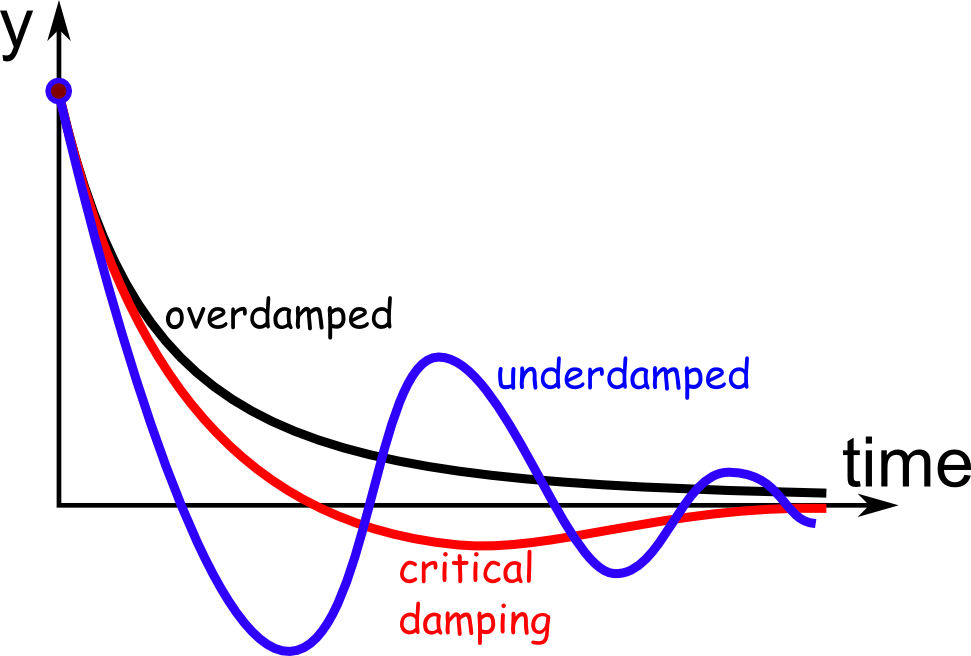
\includegraphics[width=0.6\textwidth]{./figs/SpringCases.png}
\caption{Representation of the three cases. Will be discussed in detail in the following chapter.}
\end{figure}
